
% --------------------------------------------------------------- CONFIGURATIONS

%ifdef TWOSIDE
	%\documentclass[a4paper,12pt,final,twoside,openright]{book}
%elif ONESIDE
	\documentclass[a4paper,12pt,final,oneside]{book}
%endif

\usepackage{rapport}


% -------------------------------------------------------------- META: CONSTANTS

\newcommand{\reporttitle}{Prolog}
\newcommand{\enseignants}{Jean-François~\textsc{Boulicaut}\\ Mehdi~\textsc{Kaytoue}}
\newcommand{\reportauthor}{Guillaume~\textsc{Abadie}\\ Nicolas~\textsc{Buisson}\\ Louise~\textsc{Crépet}\\ Rémi~\textsc{Domingues}\\ Aline~\textsc{Martin}\\ Martin~\textsc{Wetterwald}}
\newcommand{\hexanome}{H4404}
\newcommand{\reportsubject}{Livrable de projet}
\newcommand{\stagetopic}{Puissance 4}
\newcommand{\dateperiod}{du 1\up{er} au 15 octobre 2013}
\newcommand{\HRule}{\rule{\linewidth}{0.5mm}}
\setlength{\parskip}{1ex} % Espace entre les paragraphes

\hypersetup{
	pdftitle={\reporttitle},%
		pdfauthor={\reportauthor},%
		pdfsubject={\reportsubject},%
		pdfkeywords={INSA Lyon} {Prolog} {Puissance 4}
}

\title{\reporttitle}
\author{\reportauthor}
%\setcounter{tocdepth}{4}


% ------------------------------------------------------------------------- FILE

\begin{document}


    % ------------------------------------------------------------------- HEADER

	\renewcommand{\chaptername}{} %\renewcommand{\thechapter}{}
	\renewcommand{\contentsname}{Sommaire}

	\pagestyle{empty}
	\pagenumbering{Roman}


    % ------------------------------------------------------------ HEADER: TITLE

	% Inspiré de http://en.wikibooks.org/wiki/LaTeX/Title_Creation
\begin{center}
	\begin{minipage}[t]{0.48\textwidth}
	  \begin{flushleft}
	    
\includegraphics [width=40mm]{images/logo_INSA.png} \\[0.5cm]
			INSA Lyon\\
			20, avenue Albert Einstein\\
			69621 Villeurbanne Cedex
	  \end{flushleft}
	\end{minipage}
	\begin{minipage}[t]{0.48\textwidth}
	  \begin{flushright}
	    %\includegraphics [width=60mm]{images/logo_Passau.jpg} \\[0.5cm]
	    %Universität Passau\\
		%Innstraße, 3\\
		%	D-94032 Passau
	  \end{flushright}
	\end{minipage} \\[2cm]

	\textsc{\Large \reportsubject}\\[0.3cm]
	\HRule \\[0.4cm]
	{\Huge \bfseries \reporttitle}\\[0.3cm]
	{\LARGE \bfseries «~\stagetopic~»}\\[0.3cm]
	{\Large \dateperiod}\\[0.4cm]
	\HRule \\[1cm]

	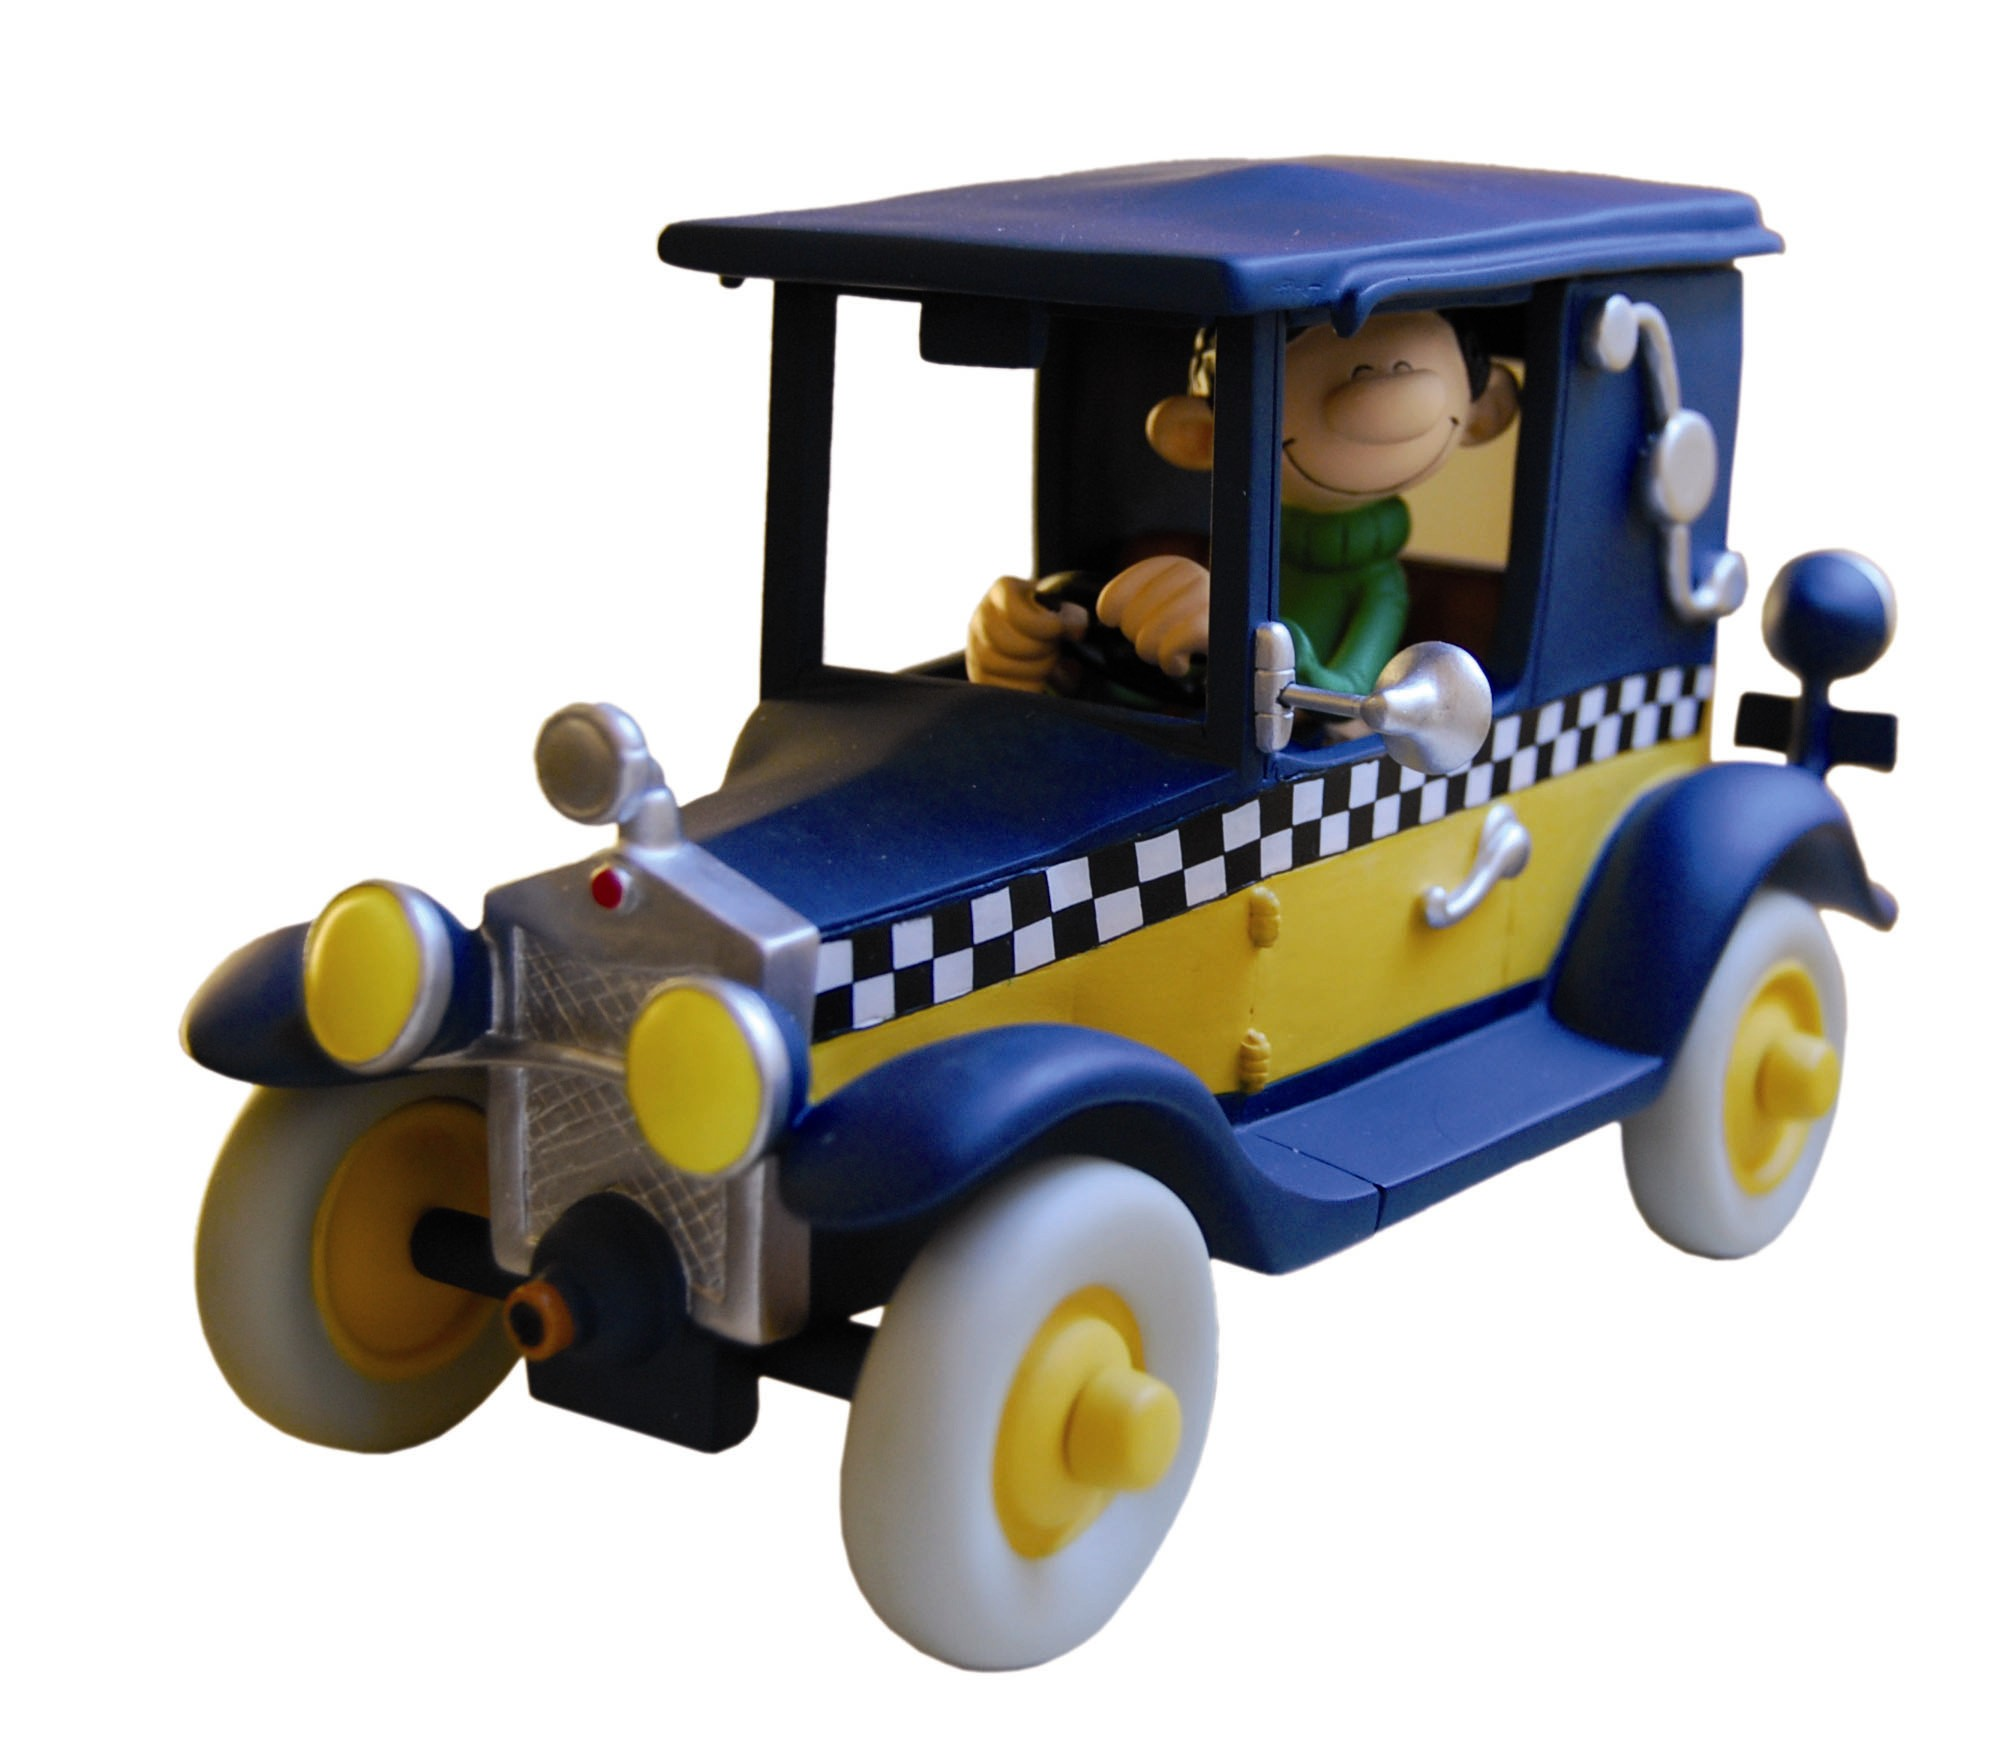
\includegraphics [scale=0.35]{images/voitureLagaffe.jpg} \\[0.7cm]
	\begin{minipage}[t]{0.4\textwidth}
	  \begin{flushleft} \large
	    \emph{Hexanôme \textbf{\hexanome}~:}\\
	    \small \reportauthor
	  \end{flushleft}
	\end{minipage}
	\begin{minipage}[t]{0.5\textwidth}
	  \begin{flushright} \large
	    \emph{Enseignants~:} \\
	    \enseignants
	  \end{flushright}
	\end{minipage}

	\vfill
	\footnotesize{Année scolaire 2013-2014}
\end{center}


	%ifdef TWOSIDE
		%\cleardoublepage
	%endif

	%\include{title2}

	%ifdef TWOSIDE
		%  \newpage
		%	\null
		%	\vfill
	%endif


    % --------------------------------------------------- HEADER: CONFIGURATIONS

	\sloppy          % Justification moins stricte : des mots ne dépasseront pas des paragraphes

    \frontmatter
		\pagestyle{empty}
		\tableofcontents
		\addtocontents{toc}{\protect\thispagestyle{empty}}

	\mainmatter
	\pagestyle{headings}

	\renewcommand{\chaptermark}[1]{\markboth{\MakeUppercase{\chaptername\ \thechapter.\ #1}}{}}
	\renewcommand{\sectionmark}[1]{\markright{\thesection{} #1}}


    % ------------------------------------------------------------------ CONTENT

    \chapter{Bilan des exercices}

\section{Prédicats}

La particularité de \texttt{Prolog} réside dans le fait qu'il n'y a pas d'itérations comme
dans un langage de programmation conventionnel~: tout n'est que prédicat. Ainsi, la
méthode de programmation est très différente. Il n'y a pas de traitement de données
dans des variables que l'on met à jour, car la programmation par prédicat permet
simplement de lier des propriétés entre des variables et/ou constantes.

\section{Vérification de propriétés}
Considérons pour la suite, le prédicat suivant~:
\[(membre(X, L) \Leftrightarrow vrai) \Leftrightarrow X \in L\]


La vérification de propriétés permet de s'assurer qu'une (ou plusieurs) constante
vérifie un ensemble de prédicats.

Considérons le code énoncé précédemment. Alors on a à l'exécution~:

\begin{lstlisting}[language=Prolog,frame=single]
?- membre(1, [1, 2, 3]).
true

?- membre(4, [1, 2, 3]).
false
\end{lstlisting}

En effet, à la première interrogation, on vérifie le prédicat $1 \in [1, 2, 3]$,
cette propriété est vérifiée, d'où la réponse de \texttt{Prolog} «~\textit{true}~». Tandis que la seconde interrogation $4 \in [1, 2, 3]$ est fausse car
$4 \notin [1, 2, 3]$, d'où la réponse «~\textit{false}~».


\section{Recherche de solutions}

La recherche de solutions consiste à définir des propriétés entre des objets et/ou constantes. Par exemple~:
\[
	X \in [1, 2, 3]
\]

\pagebreak

Ce qui en \texttt{Prolog} donne~:
\begin{lstlisting}[language=Prolog,frame=single]
?- membre(X, [1, 2, 3]).
\end{lstlisting}

Ainsi, à l'exécution, \texttt{Prolog} est capable d'évaluer les solutions de $X$ grâce à
la définition précédente du prédicat membre.

\begin{lstlisting}[language=Prolog,frame=single]
?- membre(X, [1, 2, 3]).
X = 1;
X = 2;
X = 3;
false
\end{lstlisting}

On demande à \texttt{Prolog} s'il peut prouver le prédicat fourni. Ici, il existe plusieurs manières de le prouver. Taper le caractère «\texttt{;}» permet de lui demander de prouver le prédicat d'une autre façon. Cela explique le mot \texttt{false} à la fin, signifiant qu'il est impossible de prouver ce prédicat d'une autre manière que les trois précédemment données.


\section{Recherche de solutions d'un système}

Les propriétés d'une variable par exemple, peuvent être définies par plusieurs prédicats. Par exemple~:
\[
    \left\{  
    \begin{array}{c}
        L \in [1, 2, 3]\\
        L \in [3, 4, 2]\\
    \end{array}
    \right .
\]

Peut revenir simplement en \texttt{Prolog} à
\begin{lstlisting}[language=Prolog,frame=single]
?- membre(X, [1, 2, 3]), membre(X, [3, 4, 2]).
X = 2;
X = 3;
false
\end{lstlisting}


\section{Recherche de solutions non-déterministes}

Le risque encouru lors de la recherche de solution(s), est qu'il est possible qu'une
infinité de solutions vérifie une même propriété. Considérons par exemple
le code suivant~:

\begin{lstlisting}[language=Prolog,frame=single]
?- membre(1, L).
\end{lstlisting}

Il est équivalent à $1 \in L$. Cherchons à déterminer combien de listes
pourraient vérifier cette propriété~:

\begin{description}
\item[Initialisation~:]{La liste $[1, 2]$ par exemple vérifie cette propriété.}
\item[Hérédité~:]
{
	En notant $cat(A, B)$ la concaténation de deux listes $A$ et $B$,
		\begin{itemize}
			\item soit une liste $L$ telle que $1 \in L$,
			\item alors $\forall X \in \mathbb{N}~~/~~1 \in cat([X], L)$.
		\end{itemize}
}

\item[Conclusion~:]{Il existe une infinité de solutions et \texttt{Prolog} va essayer
de toutes les générer, causant une exception due au manque de mémoire de la machine.}
\end{description}

\begin{lstlisting}[language=Prolog,frame=single]
?- membre(1, L).
L = [1|_G2214] ;
L = [_G2213, 1|_G2217] ;
L = [_G2213, _G2216, 1|_G2220] ;
L = [_G2213, _G2216, _G2219, 1|_G2223] ;
L = [_G2213, _G2216, _G2219, _G2222, 1|_G2226] ;
L = [_G2213, _G2216, _G2219, _G2222, _G2225, 1|_G2229] ;
...
\end{lstlisting}


\section{Programmation de prédicats triviaux}

Depuis le début de ce rapport, nous nous sommes contentés d'utiliser des prédicats, mais bien entendu,
l'objectif est de pouvoir en programmer soi-même. C'est ici que la méthode de programmation diffère
complètement de la programmation itérative. Nous devons procéder avec une démarche
d'analyse mathématique. Pour cela, intéressons-nous à la réécriture de~:

\[
	(membre(X, L) \Leftrightarrow vrai) \Leftrightarrow X \in L
\]

Tout d'abord, on peut remarquer que si $X$ se trouve en tête de $L$, alors il appartient de manière évidente à cette liste. Autrement dit $X \in [X, ...]$, ou encore
$X \in (L = cat([X], L1))$ avec $L1$ une autre liste. Alors on en déduit le premier prédicat~:

\begin{lstlisting}[language=Prolog,frame=single]
membre(X, [X|_]).
\end{lstlisting}

On remarque par ailleurs que si $X$ n'est pas en tête de la liste recherchée, alors il faut vérifier s'il n'est pas en tête de la sous-liste associée au retrait de cette tête, 
\[\forall (X, Y) \in \mathbb{E}^2, X \in L \Rightarrow X \in cat([Y], L)\]
Ainsi on en déduit le second prédicat~:
\begin{lstlisting}[language=Prolog,frame=single]
membre(X, [_|L]) :- membre(X, L).
\end{lstlisting}


\section{Prédicats avec calculs arithmétiques}

On se propose d'implémenter un prédicat permettant de vérifier un élement à une
position donnée dans une liste~: $X = L[I]$.

Exemple~:
\begin{lstlisting}[language=Prolog,frame=single]
?- elementAtPos(2, hello, [hi, hello, bye]).
true

?- elementAtPos(3, hi, [hi, hello, bye]).
false
\end{lstlisting}


Tout d'abord, le premier cas évident survient lorsque la liste $L$ est vide, le
prédicat doit alors être faux puisqu'aucun élément ne peut exister dans une liste vide~:
\begin{lstlisting}[language=Prolog,frame=single]
elementAtPos(_, _, []) :- fail.
\end{lstlisting}
Notez que cette ligne est facultative, car définir un prédicat comme échouant
(\texttt{fail}) revient à ne pas le définir. Nous illustrons ici simplement la démarche que nous avons suivie.

Vient ensuite le cas évident où nous voulons tester le premier élément de la liste~:
\begin{lstlisting}[language=Prolog,frame=single]
elementAtPos(1, X, [X|_]).
\end{lstlisting}

Enfin, il demeure le cas où $X$ n'est pas le premier élément. Alors, l'idée est
de récursivement prouver \texttt{elementAtPos/3}, mais en retirant le premier élément de la liste $L$ à chaque fois~:
\begin{lstlisting}[language=Prolog,frame=single]
elementAtPos(I, X, [_|L]) :- I1 is I-1, elementAtPos(I1, X, L).
\end{lstlisting}

Vous aurez remarqué ici la présence d'un index $I$ qui est décrémenté dans $I1$. En effet, le système de récursion fonctionne de telle sorte que lorsqu'une solution sera trouvée via le cas évident, si elle est trouvée, alors la valeur $I1$ de l'avant-dernier appel récursif sera égale à 1, et donc il pourra être vu comme~:
\begin{lstlisting}[language=Prolog,frame=single]
elementAtPos(I, X, [_|L]) :- 1 is I-1, elementAtPos(1, X, L).
\end{lstlisting}
Et ainsi de suite, la valeur de $I$ dépendra donc de la profondeur de la récursion nécessaire,
or comme la tête de la liste est enlevée à chaque récursion cela correspond bien à un index de la liste.

\section{Recherche avec calculs arithmétiques}

Il est alors facile d'utiliser le prédicat \texttt{elementAtPos/3} défini ci-dessus pour rechercher un élément $X$ à une position $I$ dans une liste $L$.
\begin{lstlisting}[language=Prolog,frame=single]
?- elementAtPos(2, X, [10, 11, 12]).
X = 11 ;
false
\end{lstlisting}

Cependant si nous cherchons l'index $I$ d'un élément
$X$ donné et dans une liste $L$ donnée, il survient une erreur spéciale.
\begin{lstlisting}[language=Prolog,frame=single]
?- elementAtPos(I, 12, [10, 12]).
ERROR: >/2: Arguments are not sufficiently instantiated
\end{lstlisting}

En effet si nous déroulons les prédicats, nous obtenons alors~:
\begin{lstlisting}[language=Prolog,frame=single]
elementAtPos(I, 12, [10, 12]) :- I1 is I - 1, elementAtPos(I1, 12, [12]).
elementAtPos(I, 12, [10, 12]) :- elementAtPos(I - 1, 12, [12]).
\end{lstlisting}

Nous voyons que l'expression $I - 1$ tente de vérifier une propriété liée par le prédicat
\texttt{elementAtPos/3}. Cela génère une erreur car elle est une variable non liée (\textit{unbound variable}).

En effet, cette erreur peut être facilement reproduite par~:
\begin{lstlisting}[language=Prolog,frame=single]
?- elementAtPos(I + 2, 11, [10, 11, 12]).
ERROR: elementAtPos/3: Arguments are not sufficiently instantiated
\end{lstlisting}

\section{Conditions}
En \texttt{Prolog}, il est possible de réaliser des conditions avec la syntaxe suivante~:
\begin{lstlisting}[language=Prolog,frame=single]
(condition) -> (faire quelque chose) ; (faire autre chose)
\end{lstlisting}

Codons par exemple, un prédicat liant une liste et un ensemble associé.
Trivialement, une liste vide est alors liée à un ensemble vide~:
\begin{lstlisting}[language=Prolog,frame=single]
genSet([], []).
\end{lstlisting}

Soit $L$ une liste, $S$ son ensemble associé et $X_n$ tel que $L_{n} = cat([X_n], L_{n-1})$,\\
Alors~: $S_{n} = cat([X_n], S_{n-1}) \Leftrightarrow X_n \notin S_{n-1}$ car $S_{n}$ est un ensemble.\\
D'où~:
\begin{lstlisting}[language=Prolog,frame=single]
genSet([X|L], Set) :- member(X, L), genSet(L, Set).
genSet([X|L], [X|S]) :- not(member(X, L)), genSet(L, S).
\end{lstlisting}

Remarquez alors que les deux prédicats ci-dessus sont complémentaires. Mais si nous avions
été dans un cas similaire mais plus complexe, la condition permet alors de factoriser le code, prévenant ainsi les problèmes de maintenabilité du code source~:
\begin{lstlisting}[language=Prolog,frame=single]
genSet([X|L], S) :- member(X, L) -> genSet(L, S) ; genSet(L, R), S = [X|R].
\end{lstlisting}

\section{Causalité}
Considérons le code ci-dessous générant une liste ordonnée $[N, N-1, ..., 1]$~:
\begin{lstlisting}[language=Prolog,frame=single]
generateRList([], 0).
generateRList([I|L], I) :- I1 is I - 1, generate(L, I1).
\end{lstlisting}

Ensuite essayons simplement :
\begin{lstlisting}[language=Prolog,frame=single]
?- generateRList(L, 7), sort(L, R).
L = [7, 6, 5, 4, 3, 2, 1],
R = [1, 2, 3, 4, 5, 6, 7] ;
ERROR: Out of global stack
\end{lstlisting}

En effet, \texttt{Prolog} va essayer de chercher toutes les solutions $L$ et $R$ vérifiant ce
prédicat. Alors la première solution est évidente par l'ordre des prédicats. Mais
\texttt{Prolog} va aussi essayer de chercher des solutions vérifiant cette propriété mais en commençant par évaluer
\texttt{sort}. Ce dernier étant non déterministe, l'infinité de solutions provoque un dépassement de la pile.
Mais en remplaçant un «~\texttt{,}~» (et) par un «~\texttt{->}~» (causalité), on obtient~:
\begin{lstlisting}[language=Prolog,frame=single]
?- generateRList(L, 7) -> sort(L, R).
L = [7, 6, 5, 4, 3, 2, 1],
R = [1, 2, 3, 4, 5, 6, 7].
?-
\end{lstlisting}

Ici, nous précisons que si $L$ ne vérifie pas \texttt{generateRList(L, 7)}, alors
il n'est pas la peine d'aller plus loin.


	\chapter{Projet~: Puissance~4}

\section{Règles du jeu}
Le \texttt{Puissance~4} est un jeu de société à deux joueurs. Chaque joueur doit,
chacun son tour, insérer un jeton de sa couleur dans une des sept colonnes
du plateau de jeu, chacune ayant une capacité maximale de six jetons. On peut voir chaque colonne comme
une pile de jetons, puisqu'on ne peut qu'empiler des jetons les uns sur les autres.
Le but du jeu est d'\textbf{aligner} verticalement, horizontalement ou en diagonale \textbf{4~jetons} de sa couleur avant l'adversaire.


\section{But du joueur idéal}

Dans le cas d'un joueur idéal, le but est simplement, après avoir aligné 3~jetons,
de prévoir de jouer le 4\up{ème} au tour suivant. Mais, comme l'adversaire pourrait casser la ligne en jouant à cet endroit
lors de son tour, l'objectif du joueur idéal est donc de réaliser au moins deux alignements de 3 jetons,
laissant ainsi le joueur adverse contre l'inévitable~: il ne pourra plus contrer ces alignements en un seul jeton.


\section{Travail réalisé}

En plus de l'implémentation du module du mécanisme de jeu et de la réalisation des
tests unitaires, nous avons implémenté 4 joueurs autonomes, dont une intelligence artificielle~:
\begin{itemize}

    \item joueur aléatoire~;
    \item joueur aléatoire muni d'heuristiques~;
    \item joueur parcourant l'arbre des possibilités~;
    \item intelligence artificielle apprenant par \textbf{moteur d'inférence} de ses
    échecs précédents.\\
\end{itemize}

Mais également~:
\begin{itemize}
    \item interface utilisateur en ligne de commande pour jouer une partie~;
    \item module de tournois générant des statistiques~;
    \item module d'entrainement du moteur d'inférence~;
    \item module d'étude de l'apprentissage du moteur d'inférence~;
    \item sauvegarde et chargement de la base de connaissances du moteur d'inférence.
\end{itemize}


	%\renewcommand{\chaptermark}[1]{\markboth{\MakeUppercase{#1}}{}}
	%\renewcommand{\sectionmark}[1]{\markright{#1}}

	%\addcontentsline{toc}{part}{Annexes}
	%\part*{Annexes}
	%\appendix
	%\chapter{Implémentation des exercices}

\section{Exercice 1}
\lstinputlisting[frame=single]{../exercices/exercice1.pl}

\pagebreak
\section{Exercice 2}
\lstinputlisting[frame=single]{../exercices/exercice2.pl}

\section{Exercice 3}
\lstinputlisting[frame=single]{../exercices/exercice3.pl}

\pagebreak
\section{Exercice 4}
\lstinputlisting[frame=single]{../exercices/exercice4.pl}



    % ------------------------------------------------------------------- FOOTER
\end{document}
